\documentclass[tikz, border=4pt]{standalone}
\usepackage{tikz}
\usepackage{circuitikz}
\begin{document}
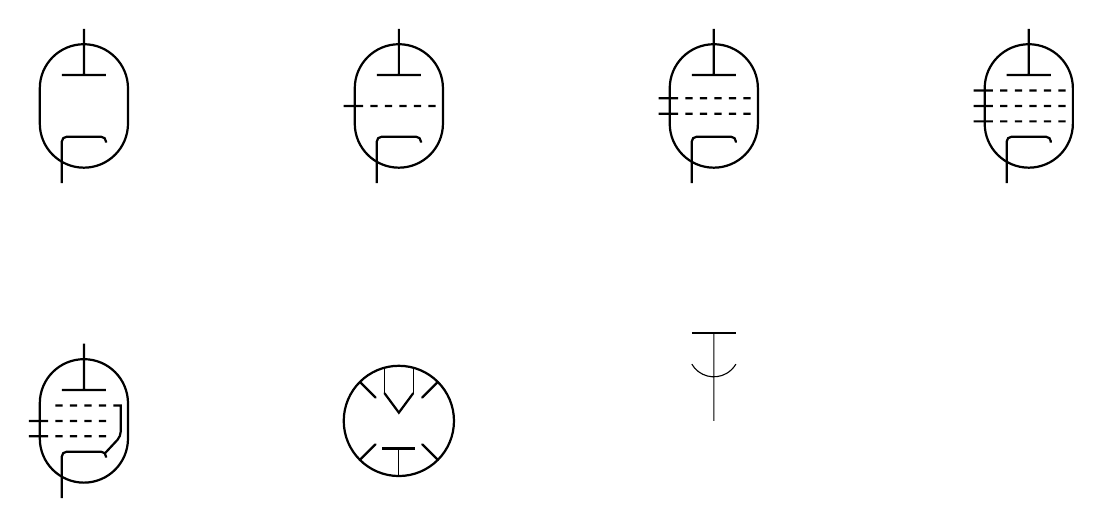
\begin{tikzpicture}[x=1cm, y=1cm]
  \begin{scope}[shift={(0,0)}, font=\large]
    \node[diodetube] at (0,0) {};
    \node[triode] at (4,0) {};
    \node[tetrode] at (8,0) {};
    \node[pentode] at (12,0) {};
    \node[pentode suppressor to cathode] at (0,-4) {};
    \node[magnetron] at (4,-4) {};
    \node[dynode] at (8,-4) {};
  \end{scope}
\end{tikzpicture}
\end{document}
